\documentclass{article}
\usepackage{graphicx}
\usepackage{amsmath}
\usepackage{amssymb}
\usepackage{listings}
\usepackage{xcolor}
\usepackage{tcolorbox}
\usepackage{caption}
\usepackage[hidelinks]{hyperref}
\setlength{\parindent}{0pt}
\usepackage[margin=0.5in]{geometry}

% For graphing
\usepackage{tikz}
\usepackage{pgfplots}
\pgfplotsset{compat=1.15}
\usepackage{mathrsfs}
\usetikzlibrary{arrows}

\usepackage{pst-plot}

\newcommand{\setExerciseNumber}[1]{%
    \begin{titlepage}
        \vbox{ }
        \vbox{ }
        \begin{center}
            % Set course here
            \includegraphics[width=0.40\textwidth]{../img/NTNU_logo.png}\\[1cm]
            \textsc{\Large TTK4135 - Optimization and Control}\\[0.5cm]
            \vbox{ }

            % Set title here
            { \huge \bfseries Exercise \##1}\\[0.4cm]

            \large
            \emph{Author:}\\
            Sondre Pedersen
            \vfill

            {\large\today}
        \end{center}
    \end{titlepage}
}

\definecolor{framecolor}{HTML}{94a3b8}
\definecolor{bgcolor}{HTML}{cbd5e1}

\newtcolorbox{problem}[2][]{
  colback=bgcolor,
  colframe=framecolor,
  fonttitle=\bfseries\color{black},
  title=Problem #2,
  width=\textwidth,
  #1
}

% Subtask 
\newcommand{\SUBTASK}[2]{\medskip\medskip\textbf{\large (#1) #2}\medskip}

% Matrix shorthand
\newcommand{\M}[1]{\begin{bmatrix} #1 \end{bmatrix}}


\begin{document}

\setExerciseNumber{1}

%%% QUESTION %%%

\begin{problem}{1: KKT example 1}
Consider
\[
  \min x_1 + 2x_2 \qquad s.t. \qquad 2 - x_1^2-x_2^2 \geq 0 ,\ x_2 \geq 0
  .\]

(a) Find the optimal point by inspecting the feasible region and the objective function.

\medskip

(b) Check the KKT conditions at the optimal point.

\medskip

(c) Illustrate the gradients of the active constraints and the objective function at the solution.

\medskip

(d) Explain why te Lagrange multipliers are positive.

\medskip

(e) Is this problem a convex problem?

\end{problem}

%%% SOLUTION %%%

\SUBTASK{a}

Here is a figure showing the feasible region in blue, f and $\nabla f$. From $\nabla f$ we can see that $x^{*} = \begin{bmatrix}
  -\sqrt{2}, 0
\end{bmatrix}^{\top}$ is the optimal point.

% Figure for 1a
\begin{center}
  \definecolor{ffqqtt}{rgb}{1.,0.,0.2}
  \definecolor{qqzzff}{rgb}{0.,0.6,1.}
  \begin{tikzpicture}[line cap=round,line join=round,>=triangle 45,x=2.0cm,y=2.0cm]
    \begin{axis}[
        x=2.0cm,y=2.0cm,
        axis lines=middle,
        xmin=-3.0,
        xmax=3.0,
        ymin=-0.5,
        ymax=2.0,
        xtick={-3.0,-2.0,...,3.0},
        ytick={-0.0,1.0,...,2.0},]
      \begin{scriptsize}
        \draw [fill=ffqqtt] (-1.4142135623730951,0.) circle (2.5pt);
        \draw[color=ffqqtt] (-0.4965675607624609,-0.03826124558724378) node {$x = (-1.41, 0)$};
        \draw[color=black] (-2.890471191856766,2.387244818114715) node {$f$};
        \draw[color=black] (0.5226191336638275,1.5418729978668009) node {$\nabla$f};
      \end{scriptsize}
      \draw [->,line width=2.pt] (0.,1.) -- (0.4,1.8);
      \draw [line width=2.pt,domain=-3.:3.] plot(\x,{(--1.-0.5*\x)/1.});
      \clip(-3.,-0.5) rectangle (3.,2.);
      \clip (axis cs:-3,0) rectangle (axis cs:3,2.0);
      \clip (0,0) circle(2.8284271247461903cm);
      \draw[line width=2.pt,color=qqzzff,fill=qqzzff,fill opacity=0.15000000596046448](-3.056385304902906,2.)--(-3.056385304902906,-0.0027082251095277743)--(4.544061207020268,-0.0027082251095277743)--(4.544061207020268,2.);
      \draw [rotate around={0.:(0.,0.)},line width=2.pt,color=qqzzff,fill=qqzzff,fill opacity=0.15000000596046448] (0.,0.) ellipse (2.8284271247461903cm and 2.8284271247461903cm);
    \end{axis}
  \end{tikzpicture}
\end{center}

\SUBTASK{b}

The Lagrangian is $\mathcal{L}(\mathbf{x, \lambda}) = x_1 + x_2 - \lambda_1(2 - x_1^2 - x_2^2) - \lambda_2(x_2)$.

The KKT-conditions are in this case \begin{align}
  \nabla _x \mathcal{L}(\mathbf{x, \lambda}) &= 
  \begin{bmatrix}
    1 \\ 2  
  \end{bmatrix}
  + \lambda_1
  \begin{bmatrix}
    2x_1 \\ 2x_2
  \end{bmatrix}
  - \lambda_2
  \begin{bmatrix}
    0 \\ 1
  \end{bmatrix}
  = 0
  \\
  c_1(\mathbf{x}) &= 2-x_1^2 - x_2^2 \geq 0 \\
  c_2(\mathbf{x}) &= x_2 \geq 0 \\
  \mathbf{\lambda} \geq 0 \\
  \lambda_1c_1(\mathbf{x}) &= 0 \\
  \lambda_2c_2(\mathbf{x}) &= 0
\end{align}.

(2), (3), (5), and (6) are satisified since both conditions are binding ($c_1(\mathbf{x^*}) = c_2(\mathbf{x^*}) = 0$).

(1) and (4) are satsified when $\lambda_1 = \frac{\sqrt{2}}{4}$ and $\lambda_2 = 2$
%%% QUESTION %%%

\begin{problem}{Problem 2: Linear programming problem}
  In a plant three products, R, S, and T are made in two process stages A and B. 
  To make a product the following time in each process stage is required: 
  \begin{itemize}
    \item 1 tonne of R: 3 hours in stage A plus 2 hours in stage B. 
    \item 1 tonne of S: 2 hours in stage A and 2 hours in stage B. 
    \item 1 tonne of T: 1 hour in stage A and 3 hours in stage B.
  \end{itemize}
  During one year, stage A has 7200 hours and stage B has 6000 hours available production time. 
  The rest of the time is needed for maintenance. It is required that the available production time should be fully utilized in both stages.
  
  \medskip The profit from the sale of the product is: 
  \begin{itemize}
    \item R: 100 NOK per tonne.
    \item S: 75 NOK per tonne.
    \item T: 55 NOK per tonne.
  \end{itemize}
  We wish to mazimize the yearly profit.

  
  \medskip (a) Formulate this as an LP problem on standard form.
  
  \medskip (b) Which basic feasible points exist?
  
  \medskip (c) Find the solution by checking the KKT conditions at all the feasible points found in (b).
  
  \medskip (d) Formulate the dual problem for the LP in (a). 
  
  \medskip (e) Show that the optimal objective function value for the LP in (a) equals the optimal objective 
  function value for the dual problem in (d) by showing that $c^{\top}x^* = b^{\top}\lambda^*$.
  
  \medskip (f) If you can make either stage A or stage B more available, which should you choose?


\end{problem}

%%% SOLUTION %%%

%%% QUESTION %%%

\begin{problem}{3: Second-order conditions}
Consider
\[
  \min_{x \in \mathbb{R}^{2}} f(x) = -2x_1 + x_2 \qquad s.t. \qquad 
  \left\{
    \begin{aligned}
      c_1(x) &= (1-x_1)^2 - x_2 \geq 0 \\
      c_2(x) &= x_2 + 0.25x_1^2 - 1 \geq 0
    \end{aligned}
    \right
.\] 

The optimal solution is $x^{*} = (0, 1)^{\top}$, where both constraints are active. 

\medskip

(a) Do the LICQ hold at this point?

\medskip

(b) Are the KKT conditions satisfied?

\medskip

(c) Write down the sets $\mathcal{F}(x^{*})$ and $\mathcal{C}(x^{*}, \lambda^{*})$.

\medskip

(d) Are the second-order necessary conditions satisifed?


\end{problem}


%%% SOLUTION %%%

%%% QUESTION %%%

\begin{problem}{4: Find optimizers}
Find the \textit{maxima} of the function $f(x) = x_1x_2$ over the unit disc defined by the inequality constraint $x_1^2 + x_2^2 = 1$. Illustrate the gradients of the
active constraint and the objective function at the optimal points.
\end{problem}

%%% SOLUTION %%%

\begin{align*}
  \mathcal{L}(\mathbf{x}, \lambda)        & = x_1x_2 - \lambda_1(x_1^2 + x_2^2-1)                   \\
  \nabla \mathcal{L}(\mathbf{x}, \lambda) & = \M{x_2 -2\lambda x_1                                  \\ x_1 - 2\lambda x_2 \\ -x_1^2 -x_2^2 + 1} = 0 \\
  \implies x_1                            & = x_2 = \pm \frac{1}{\sqrt{2}},\  \lambda = \frac{1}{2}
\end{align*}

\begin{center}
  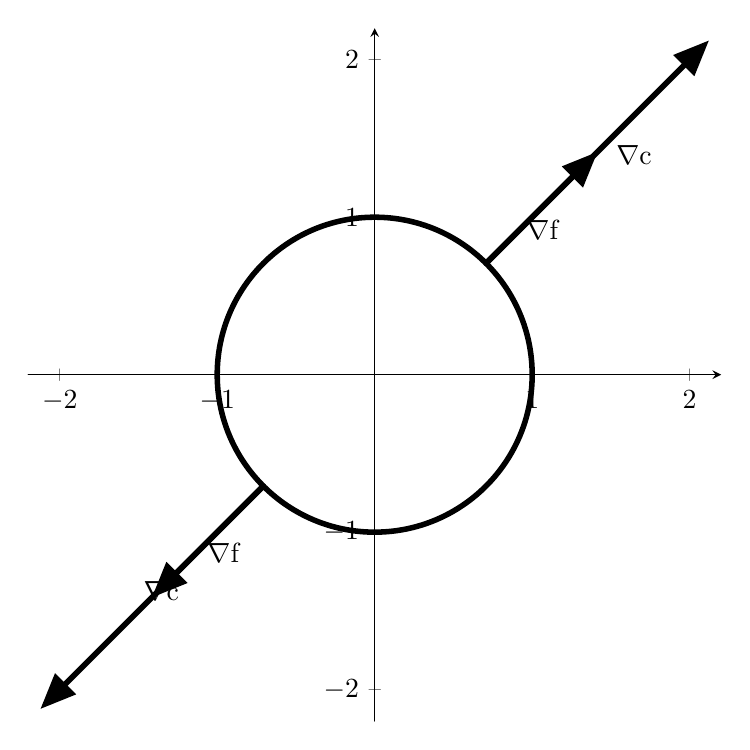
\begin{tikzpicture}[line cap=round,line join=round,>=triangle 45,x=2.0cm,y=2.0cm]
    \begin{axis}[
        x=2.0cm,y=2.0cm,
        axis lines=middle,
        xmin=-2.2,
        xmax=2.2,
        ymin=-2.2,
        ymax=2.2,
        xtick={-2.0,-1.0,...,2.0},
        ytick={-2.0,-1.0,...,2.0},]
      \clip(-2.2,-2.2) rectangle (2.2,2.2);
      \draw [line width=2.pt] (0.,0.) circle (2.cm);
      \draw [->,line width=2.pt] (0.7071067811865475,0.7071067811865475) -- (1.414213562373095,1.414213562373095);
      \draw [->,line width=2.pt] (-0.7071067811865475,-0.7071067811865475) -- (-1.414213562373095,-1.414213562373095);
      \draw [->,line width=2.pt] (0.7071067811865475,0.7071067811865475) -- (2.1213203435596424,2.1213203435596424);
      \draw [->,line width=2.pt] (-0.7071067811865475,-0.7071067811865475) -- (-2.1213203435596424,-2.1213203435596424);
      \begin{scriptsize}
        \draw[color=black] (1.0637954312887226,0.9162861268834652) node {$\nabla$f};
        \draw[color=black] (-0.961618466685309,-1.1309820687316112) node {$\nabla$f};
        \draw[color=black] (1.6466483515690196,1.397139155035049) node {$\nabla$c};
        \draw[color=black] (-1.3550441878745096,-1.3714085828074032) node {$\nabla$c};
      \end{scriptsize}
    \end{axis}
  \end{tikzpicture}
\end{center}

\end{document}
